\documentclass{article}

\usepackage[most]{tcolorbox}
\usepackage{physics}
\usepackage{graphicx}
\usepackage{amsmath}
\usepackage{amssymb}
\usepackage{float}


\usepackage[utf8]{inputenc}
\usepackage[a4paper, margin=1in]{geometry} % Controla los márgenes
\usepackage{titling}

\title{Clase 5 }
\author{Manuel Garcia.}
\date{\today}

\renewcommand{\maketitlehooka}{%
  \centering
  \vspace*{0.05cm} % Espacio vertical antes del título
}

\renewcommand{\maketitlehookd}{%
  \vspace*{2cm} % Espacio vertical después de la fecha
}

\newcommand{\caja}[3]{%
  \begin{tcolorbox}[colback=#1!5!white,colframe=#1!25!black,title=#2]
    #3
  \end{tcolorbox}%
}

\begin{document}
\maketitle

\section{Primera forma fundamental en una superficie }
\caja{green}{Tangente a la curva }{
  \begin{gather}
    \frac{d r }{d t} = r_u \dot u + r_v \dot v \quad r_u = \frac{\partial r }{\partial u} = (x_u,y_u,z_u) \quad r_v = \frac{\partial r }{\partial v} = (x_v,y_v,z_v) 
  \end{gather}
  $ \frac{\partial r }{\partial u}, \frac{\partial r }{\partial v} $ son linealmente independientes de acuerdo a las condiciones de regularidad de la superficie.
}

\caja{green}{Longitud de una curva en la superficie parametrizada por u y v}{
  Recordemos que $ r(u,v) = (x(u,v), y(u,v), z(u,v)) $
  \begin{gather}
    dl ^2 = \left|v ^2\right|dt ^2 = ( \dot x ^2+ \dot y ^2 + \dot z ^2 )dt ^2\\
    \text{Usando }r(u,v) \qquad \dot x = x_u \dot u + x_v \dot v, \quad \dot y = y_u \dot u + y_v \dot v, \quad \dot z = z_u \dot u + z_v \dot v\\
    dl ^2 = \left|v ^2\right|dt ^2 = (E\dot u ^2 + 2F \dot u \dot v + G \dot v)dt ^2\\
    \rightarrow g _{ij } dx ^ {i } dx ^ {j } = Edu ^2 + 2F dudv + Gdv ^2, \qquad donde \quad x ^ {1 } = u, x ^ {2 } = v 
  \end{gather}
  \tcblower
  \textbf{Primera forma fundamental o métrica inducida en la superficie }
  \begin{gather}
     g _{ij } (u,v ) = \bra{\frac{\partial r }{\partial x ^ {i }}}\ket{\frac{\partial r  }{\partial x ^ {j }}}, \text{ Donde } (x ^ {1 }, x^ {2} )  = (u,v)\\
     g _{ij } (u,v) = \begin{bmatrix}
         E & F \\
         F & G
     \end{bmatrix} \\
     g _{11 }  = E = x_u ^ {2 }+ y_u^2 + z_u^2 \\
     g_{22} = F = x_ux_v + y_u y_v + z_uz_v\\
     g _{33 }  = G = x_v^2 + y_v^2 + z_v^2\\
     (\dot x ^2 + \dot y ^2 + \dot z ^2)dt ^2 = Edu ^2 + 2 F dudv + G dv ^2
  \end{gather}
}
\textbf{Ejemplo} Si la superficie se representa por $ z = f\left(x,y \right) $, entonces $ x=u, \quad y = v  $, entonces la escribiremos como $ r\left(x,y\right)=(x,y, z\left(x,y\right)) $: 
\begin{gather}
  r_x  = (1,0,f_x), \qquad r_y  = (0,1, f_y)\\
  E = \bra{r_x }\ket{r_x } = 1+ f_x ^ {2 }\\
  F = \bra{r_x }\ket{r_y } = f_xf_y\\
  G = \bra{r_y }\ket{r_y } = 1+ f_y ^2\\
  g _{ij }  = \bra{r _{x ^ {i }} }\ket{r _{x ^ {j }} } =  \begin{bmatrix}
      1+ f_x ^2 & f_x f_y  \\
      f_x f_y  & 1+f_y ^2
  \end{bmatrix} \quad \rightarrow\quad ds ^2 = (1+ f_x ^2)dx ^2 + 2 f_xf_y dxdy + (1+ f_y ^2)dy ^2
\end{gather}

\textbf{Ejemplo } Si la superficie se representa por $ F\left(x,y,z \right)=0  $, por el teorema de la función implicita, localmente, entorno a un punto regular, podemos encontrar $ z = f\left(x,y\right) $ y calcular sus derivadas de acuerdo al teorema de la función implícita: 
\begin{gather}
  F\left(x,y,z\right)=0\qquad \text{ Podemos suponer que  }\quad F\left(x,y,f\left(x,y\right)\right)=0, \quad z = f\left(x,y\right)\\
  \text{Teo. func. implicita } f_x  = - \frac{\frac{\partial F }{\partial x}}{\frac{\partial F }{\partial z}} = - \frac{F_x }{F_z }, \quad f_y = - \frac{F_y }{F_z}\\
  g _{ij }  = \begin{bmatrix}
      1+ \left(\frac{F_x }{F_z }\right)^2 & \frac{F_x F_y }{F_z ^2} \\
      \frac{F_x F_y }{F_z ^2} & 1+ \left(\frac{F_y }{F_z }\right)^2
  \end{bmatrix} = \left(\delta _{ij } + \frac{F_i F_j }{F_z ^2}\right) 
\end{gather}

\textbf{Cilindro } $ f\left(x,y\right)=0  $, $ z  $ arbitrario.
\begin{gather}
  ds ^2 = dl ^2 + dz ^2 
\end{gather}
Notemos que se introdujeron unas nuevas corrdenadas $ (l,z) $ las cuales son euclideanas. 
\begin{gather}
  g\left(l,z\right)=\begin{bmatrix}
      1 & 0 \\
      0 & 1
  \end{bmatrix}   
\end{gather}

\textbf{Ejemplo cilindro } $ f\left(x,y\right)=x ^2 + y ^2 -1 = 0  $ esto lo podemos parametrizar utilizando $ \sin{u}, \cos{u } $.
\begin{figure}[H]
  \begin{center}
    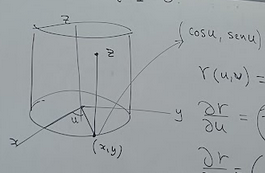
\includegraphics[width=0.3\textwidth]{cilindro.png}
  \end{center}
\end{figure}

\begin{gather}
  (\cos{u }, \sin{u })\\
  r\left(u,v\right)=\begin{bmatrix} \cos{u } & \sin{u } & v \end{bmatrix}\\
  \frac{\partial r  }{\partial u } = \begin{bmatrix} \sin{u } & \cos{u } & 0  \end{bmatrix}\\
  \frac{\partial r  }{\partial v } = \begin{bmatrix} 0  & 0  & 1 \end{bmatrix}\\
  g _{11}  = \bra{r_u }\ket{r_u } = 1 = E\\
  g _{12 }  = \bra{r_u }\ket{r_v } = 0 = F  \\
  g _{22 }  = \bra{r_v }\ket{r_v } = 1 = G \\
  \rightarrow \quad g _{ij }  = \begin{bmatrix}
      1 & 0 \\
      0  & 1
  \end{bmatrix}  
\end{gather}

\section{Area de una superficie }
Si $ U  $ es una región del plano $ xy  $: 
\begin{gather}
  \sigma (U) = \int \int_{U }^{} dxdy\\
\end{gather}
Si transformamos la región U en $ r(U) = V  $ através del mapa $ x(u,v), y(u,v) $, el área será:
\begin{gather}
   \sigma (U) = \int \int_{v }^{} \left|J \right|dudv = \int \int_{V }^{} \left|x_uy_v - x_vy_u\right|dudv
\end{gather}
\caja{green}{Definicion }{
  El área d ela usperficie mapeada por $ r(u,v) $ es: 
  \begin{gather}
    \sigma(U) = \int \int_{U }^{}\sqrt{g } du dv 
    \label{eq:def_area}
  \end{gather}
  Donde $ g = det(g _{ij } ) = det \begin{bmatrix}
      E & F \\
      F & G
  \end{bmatrix} = EG- F ^2  $
}

\hfill

\textbf{Ejemplo } Imaginemos que tenemos un paralelogramo y sus lados están dados por los vectores $ \xi, \eta  $. Su area la podemos describir como un determinante $ A = \begin{bmatrix}
    \xi ^ {1 } & \xi ^ {2 } \\
    \eta ^ {1 } & \eta ^ {2 }
\end{bmatrix} \rightarrow det(A) = \xi ^ {1 } \eta ^ {2 } - \xi ^ {2 } \eta ^ {2 }  $. Esto lo podemos describir como: 
\begin{gather}
  \sigma (\xi, \eta ) = \left|\xi \cross \eta \right| = det(A)\\
  \xi = \xi ^ {1 }e_1 + \xi ^ {2 }e_2 \qquad \qquad e_1 = \begin{bmatrix} 1  & 0  \end{bmatrix}, \qquad e_2 = \begin{bmatrix} 0  & 1  \end{bmatrix} \\ 
  \eta = \eta ^ {1} e_1 + \eta ^ {2 }e_2
\end{gather}
Podemos definir: 
\begin{gather}
  g _{11} = \bra{\xi }\ket{\xi } = (\xi ^ {1 }) ^ {2 } + (\xi ^ {2 })^2\\
  g _{12} = \bra{\xi }\ket{\xi } = \xi ^ {1 }\eta ^ {1 }+ \xi ^ {2 } \eta ^ {2 }\\
  g _{22} = \bra{\eta }\ket{\eta } =   (\eta ^ {1 }) ^ {2 } + (\eta ^ {2 })^2\\
  g _{ij }  = \begin{bmatrix}
      \xi ^ {1 } & \xi ^ { 2 } \\
      \eta ^ {1 } & \eta ^ {2 }
  \end{bmatrix} \begin{bmatrix}
      \xi ^ {1 } & \eta ^ {1 } \\
      \xi ^ {2 } & \eta ^ {2 }
  \end{bmatrix} = A A ^ {T}\\  
  det(g _{ij } ) = det(A) det(A ^ {T }) = (det A) ^ {2 }\\
  det(A) = \sqrt{det(g _{ij } )} = \sqrt{g } 
\end{gather}

\textbf{Ejemplo } $ z = f\left(x,y\right) $ su metrica (la calculamos anteriormente): $ g _{ij }  = \begin{bmatrix}
    1+ f_x ^ {2 } & f_x f_y  \\
    f_x f_y  & 1+ f_y ^ {2 }
\end{bmatrix}   $ y $ g = ((1+ f_x ^ {2 })(1+ f_y ^ {2 }) - f_x to
2 f_y ^ {2 }) = [1 + f_x ^ {2} + f_y ^ {2 }] $. 
\begin{gather}
  \sigma (u) = \int \int_{v }^{} \sqrt{1+ f_x ^ {2 }+ f_y ^ {2 }} dxdy
\end{gather}
\textbf{Ejemplo } $ F\left(x,y,z\right)=0  $
\begin{gather}
  g = \left[1 + \frac{F_x ^ {2 }}{f_z ^2} + \frac{F_y ^ {2 }}{F_z ^2}\right] = \frac{F_z ^2 + F_x ^2 + F_y ^2 }{F_z ^2} = \frac{(\grad F) ^2}{F_z ^2} \rightarrow \sqrt{g} = \frac{|\grad F |}{|F_z|}\\
  \sigma (u) = \int \int_{v }^{} \frac{|\grad F| }{|F_z| }dxdy
\end{gather}

\section{Segunda forma fundamental en una superficie }
Entorno a un punto regular $ P_0  = \begin{bmatrix} x_0  & y_0  & z_0  \end{bmatrix} $ se puede describir una superficie por medio de $ z = f\left(x,y\right) $, de tal manera que el eje z sea perpendicular a la superficie en ese punto. De esta forma $ \grad f= 0 |_{P_0 } $, ya que la 1ra variación de la función es cero, a continuación se toma la segunda variación: 
\begin{gather}
  d ^2 f = f _{xx } dx ^2 + 2 f _{xy } dxdy + f _{yy } dy ^2 
\end{gather}
Matrix Hessiana: 
\begin{gather}
  H _{ij }  = \begin{bmatrix}
      f _{xx }  & f _{xy }  \\
      f _{xy }  & f _{yy } 
  \end{bmatrix} \qquad \qquad H _{ij } = H _{ji}\\
  \text{Hessiano } \quad \rightarrow \quad \text{Curvatura}\\
  d ^2f = \begin{bmatrix} dx  & dy  \end{bmatrix} \begin{bmatrix}
      f _{xx }  & f _{xy }  \\
      f _{yx } & f _{yy } 
  \end{bmatrix} \begin{bmatrix}
      dx  \\
      dy   
  \end{bmatrix}   
\end{gather}

\end{document}
